\documentclass[ ngerman, fontsize= 12pt, paper=a4, headings=big, titlepage=true]{article}

%Sprache
\usepackage{babel}
\usepackage[utf8]{inputenc}
\usepackage[T1]{fontenc}
\usepackage{mathptmx}
\usepackage{hyperref}
\usepackage{lmodern, microtype}
\usepackage{csquotes}
\usepackage{hyperref}
\usepackage{enumerate}
%\usepackage[numbers,round]{natbib}
\usepackage[backend=bibtex,               % biber als Sortierprogramm (bibtex)
sortlocale=de,               % deutsche Sortierung (Sonderzeichen)
abbreviate=false,            % keine Abkürzungen benutzen
natbib=true,                 % natbib-ähnliche Befehle verfügbar
%bibstyle=authortitle,        % Stil ohne Label, z.B. [1]
%citestyle=authoryear,        % Autor-Jahr-Zitate
language=auto,               % Hauptsprache des Dokuments
babel=other,                 % berücksichtigt hyphenation-Feld in der .bib
maxcitenames=2,              % ab 2 Namen et al. bzw. u.a.
maxbibnames=10,              % ab 10 Namen im Verzeichnis et al. bzw. u.a.
block=nbpar,                 % Quallenangabe als Block je item
isbn=false,                  % keine ISBN
url=true,                   % keine URL
doi=false,                   % keine DOI
eprint=false]{biblatex}

%\usepackage[onehalfspace]{setspace}
%Tablellen:
\usepackage{multirow}
\usepackage{caption}
\usepackage{booktabs}
\usepackage{rotating}
\usepackage{hhline,float}
%\usepackage{pdfpages}

%Mathematik
\usepackage{amsmath}
\usepackage{amsfonts}
\usepackage{amssymb}
\usepackage{mathtools}
\usepackage{bbm}

%Grafik
\usepackage{wrapfig}
\usepackage{color}
\usepackage[svgnames]{xcolor}
\usepackage[
left=3cm,
right=2cm,
top=2.5cm,
bottom=2cm,
%includeheadfoot
]{geometry}

%R-Code
\usepackage{listings}
\lstset{language=R,
	basicstyle=\small\ttfamily,
	stringstyle=\color{DarkGreen},
	otherkeywords={0,1,2,3,4,5,6,7,8,9},
	morekeywords={TRUE,FALSE},
	deletekeywords={data,frame,length,as,character},
	keywordstyle=\color{blue},
	commentstyle=\color{DarkGreen},
}



%\bibliographystyle{natstat} 
\addbibresource{Literatur.bib} 
\setlength{\bibitemsep}{0.5\baselineskip}
\setlength{\bibhang}{2em}
\begin{document}
	
	
	\begin{center}
		\Large
		Technische Universität Dortmund\\
		Fakultät Statistik\\
		Sommersemester 2021\\
		
		\vspace{4em}
		
		Grundlagen der Versuchsplanung: Bericht über das 2.Experiment
		
		\Huge
		\textbf{Temperaturexperiment}
		
		\Large
		\vspace{5em}
		Dozenten:\\
		JProf. Dr. Kirsten Schorning, M.Sc. Onur Gül, B.Sc. Wiebke Dammann\\
		
		
		\vspace{8em}
		Autorinnen: \\
		Kaya Maria Bayer\\
		Ketevan Gurtskaia\\
		Danuscha Große-Hering\\	
		Alicia Hemmersbach\\
		
		
		
		\vspace{12em}
		
		05.Juli 2021
		
	\end{center}
	
	\newpage	
	
	\tableofcontents
	\newpage
	
	\section{Einleitung}
	Ein Thermometer besitzen vermutlich die meisten Haushalte. Einige davon besitzen wahrscheinlich auch ein Thermometer, welches die Temperatur draußen und drinnen messen kann. Möglicherweise hat man sich bereits die Frage gestellt, worin der Unterschied zwischen dem Innen- und Außensensor dieser Thermometer liegt und ob dieser lediglich darin besteht, dass Außensensoren wetterfest sind, oder ob beide Sensoren, unabhängig von weiteren äußeren Einflüssen, die gleichen Temperaturen messen würden, wenn man den Innensensor nach außen und den Außensensor nach innen legt. \newline 
	
	Genau dieser Frage wird in dem folgenden Temperaturexperiment nachgegangen. Es soll überprüft werden, ob es Unterschiede bei den Messungen der beiden Sensoren drinnen und draußen gibt. \newline
	
	Dazu sollen mit 10 gleichen Thermometern einige Messungen drinnen und draußen durchgeführt werden. Hierbei wird dann der Unterschied der zwei gemessenen Temperaturen zwischen Innen- und Außensensor ausgewertet und mit Hilfe eines statistischen Tests interpretiert. \newline 
	
	Im Folgenden wird auf die Problemstellung des Experiments und die Versuchsbedingungen, dann auf die Analyse des Problems, das zugehörige statistische Modell, die Hypothesen, die statistischen Auswertungsmethoden des Experiment und die Versuchsplanung eingegangen.
	
	\section{Problemstellung und Versuchsbedingungen}
	Ziel des Experimentes ist es, herauszufinden, ob die Messungen der Innen- und Außensensoren am selben Ort bei gleicher Temperatur übereinstimmen, oder ob es Unterschiede gibt. Außerdem soll untersucht werden, ob es einen Unterschied macht, ob draußen oder drinnen gemessen wird.\newline
	
	Um diese beiden Fragestellungen zu beantworten, sollen insgesamt 6 Messungen mit jeweils 10 Thermometern, die einen Außen- und einen Innensensor haben, durchgeführt werden, sodass nach der Durchführung des Experimentes 120 Messwerte vorliegen. Dabei sollen alle Thermometer gleich alt und zudem möglichst neu sein. Außerdem dürfen die Thermometer keine sichtbaren oder bekannten Schäden haben. Die Messungen werden in 2 Zeitslots über einen Tag verteilt, an dem keine extremen Wetterbedingungen herrschen, vorgenommen.  Außerdem werden die Thermometer vor jeder Messung randomisiert in 2 Gruppen mit jeweils 5 Thermometern aufgeteilt. Die eine Gruppe der Thermometer misst die Temperatur draußen und die andere Gruppe der Thermometer misst die Temperatur drinnen. Der Raum, in welchen die Innenmessungen stattfinden, soll hierbei keine angeschaltete Heizung oder Klimaanlage haben. Außerdem sollen, falls vorhanden, alle Fenster geschlossen und soweit abgedunkelt sein, dass keine direkte Sonneneinstrahlung, zum Beispiel durch Fenster, auf die Thermometer trifft. \newline
	
	Die Messungen draußen sollen an einem windgeschützten Ort ohne direkte und auch ohne gespiegelte Sonneneinstrahlung, zum Beisiel durch Wasser, stattfinden. Außerdem sollten die Thermometer an einem trockenen Ort platziert werden und es sollten andere direkte Wärmequellen mindestens 10 Meter Abstand von dem Messort haben. \newline
	
	Für die Messungen werden die 5 Thermometer draußen und die 5 Thermometer drinnen jeweils nebeneinander auf einen ebenen identischen Tisch gelegt. Außerdem ist darauf zu achten, dass die Innen- und Außensensoren direkt nebeneinander liegen.  \newline
	
	Es werden jeweils 3 Messungen pro Thermometer in 2 Zeitslots durchgeführt. Der erste Slot ist von 4:00 - 6:00 Uhr und der zweite Slot von 16:00 - 18:00 Uhr. Insgesamt beträgt jeder Zeitslot zwei Stunden. Zu Beginn der Zeitslots werden die Thermometer für 15 Minuten in den Kühlschrank gelegt. Somit wird die Temperatur von allen Thermometern gleichmäßig neutralisiert. Nach Ablauf der 15 Minuten werden die Thermometer dann von 2 Versuchsleitern aus dem Kühlschrank entnommen und auf dem dafür vorgesehenen Tisch platziert. Dabei ist ein Versuchsleiter für die Thermometer draußen und ein Versuchsleiter für die Thermometer drinnen zuständig. Die Thermometer sollen jeweils 20 Minuten auf dem Tisch liegen und sich der jeweiligen Temperatur anpassen, bevor die angezeigten Temperaturen von den anderen beiden Versuchsleitern abgelesen und notiert werden. Nach der ersten Messung in beiden Slots kommen alle Thermometer für 15 Minuten zurück in den Kühlschrank, damit sich die Temperatur erneut neutralisieren kann. Nach Ablauf der 15 Minuten werden die Thermometer wieder von den ersten beiden Versuchsleitern auf dem Tisch platziert. Darauf hin werden die Temperaturen 20 Minuten abgelesen und notiert. Die dritte Messung in beiden Zeitslots läuft nach dem gleichen Schema so ab. Es ist zu beachten, dass das Ablesen und Notieren der Werte möglichst schnell passiert, damit alle 5 Werte jeweils zur gleichen tatsächlich herrschenden Temperatur abgelesen werden. In der möglicherweise verbleibenden Zeit der Slots und zwischen dem ersten und zweiten Slots können die Thermometer jeweils auf den Tischen liegen bleiben, wobei auch hierbei darauf zu achten ist, dass sie in der Zwischenzeit keinem Regen oder anderen Wetterextrema ausgesetzt sind.
	
	
	
	\section{Analyse des Problems}
	
	%was ist die interessiernde abhängige Variable?
	Es soll untersucht werden, ob die Messungen der Innen-und Außensensoren der Thermometer gleich sind, ist die vorliegende interessierende Variable die Temperaturdifferenz der Innen-und Außensensoren:\\
	\begin{center}
		%$y_{\text{Differenz}} = y_{\text{Außensensor}}-y_{\text{Innensensor}} $
		$y_{\text{\tiny{Differenz}}} = y_{\text{\tiny{Außensensor}}}-y_{\text{\tiny{Innensensor}}} $
	\end{center}
	
	%Was ist die interessierende Einflussvariable udn wie können diese variiert werden?
	Die wahre Temperatur ist eine Einflussvariable. Diese können wir jedoch nicht kontrollieren.  Zudem ist auch der Ort des Thermometers eine interessierende Einflussvariable, welche wir kontrollieren können. In dem Versuch werden wir zwei feste Orte festlegen: Innerhalb und Außerhalb eines Gebäudes. \\
	
	%Was sind mögliche Störvariablen und welche können kontrolliert werden?
	
	Im Folgenden werden mögliche Störvariablen genannt und inwiefern man diese kontrollieren kann. Generell haben die Wetter-bzw. die Klimabedingungen einen hohen Einfluss auf den Versuch.  In geschlossenen Räumen ist dies die Nutzung einer Heizung oder Klimaanlage und die Luftfeuchtigkeit. Die Klimabedingungen im Raum werden Konstant gehalten. Das bedeutet, dass sowohl die Klimaanlage, wie auch die Heizung oder Anlagen zur Regulierung der Luftfeuchtigkeit, ausgeschaltet werden. Außerhalb eines Gebäudes fällt auch die Luftfeuchtigkeit, die Sonnenbestrahlung an dem Messort, die Windstärke, wie auch Regen darunter. Auch diese Bedingungen möchten wir möglichst konstant halten. Dies wird umgesetzt, indem die Thermometer an windgeschützten und überdachten ohne direkter Sonnenbestrahlung platziert werden sollen. Neben diesen Wetterfaktoren, kann auch das Thermometer einen Einfluss haben. Zum einen können Messungenauigkeiten zwischen unterschiedlichen Gererätehersteller oder Modellen zusätzlich zu den Messungenauigkeiten der einzelnen Thermometer dazukommen. Dies würde dazu führen, dass unser Versuch komplizierter würde. Deswegen halten wir das Modell des Thermometers konstant. Zudem ist die Tageszeit bzgl. der unterschiedlichen Temperaturen am Tage eine Störvariable. \\
	
	%Von welchen Störvariablen soll noch der Einfluss erfasst werden?
	Zusammengefasst sollen die meisten Störvariablen möglichst konstant gehalten werden und somit soll dessen Einfluss nicht erfasst werden. Jedoch können wir sie Messzeiten beeinflussen.  \\
	
	%Welche Störvariablen sollen als Blockvariablen aufgefasst werden?
	Durch die Variation der Messzeiten ist eine Variation der Temperatur möglich. Das bedeutet genauer: Zur Zeit des Sonnenaufgangs ist es tendenziell kälter, als zur Nachmittagszeit. \cite{WK2}. Deswegen wird die Messzeit als Blockvariable mit zwei Stufen aufgefasst. Dabei  entspricht die erste Stufe die Morgenstunden und die zweite Stufe die Nachmittagsstunden. 
	
	
	
	\section{Modell, Hypothesen und statistische Auswertungsmethoden}
	Nach der Durchführung des Experiments liegen die Versuchsergebnisse zur Auswertung vor. \\
	60 Messwerte der Innensensoren:  $ V^a_{1}, ...V^a_{30}, V^i_{31}, ... V^i_{60} $   \\
	60 Messwerte der Außensensoren:  $ W^a_1, ...W^a_{30},W^i_{31},..., W1 i_{60} $ \\
	wobei $a \hat{=}$ Messungen außerhalb des Gebäudes,   $i \hat{=} $ Messungen im Gebäude, jeweils 30 Beobachtungen für alle vier Kombinationen $\{$Außensensor, Innensensor$\} \times \{$Draußen, Drinnen$\} $. Stichprobenumfang n ist 60, Versuchsumfang N ist $2 \cdot n =120 $. \\
	
	Da es in diesem Experiment sich um verbundene Stichproben handelt (die Paare $ ( V_j, W_j ), j = 1,...60 $ sind bivariate Zufallsvektoren von Messungen der Innen- und Außensensoren eines Thermometers), werden die Differenzen $ X_j := W_j - V_j,$ mit  $j = 1, .., 60, $, unter der Voraussetzung, dass die Einzelwerte repräsentativ für die beiden Arten des Sensors sind, betrachtet(für die erste Fragestellung ist es nicht relevant, wo die Messung stattgefunden hat, deswegen werden hier die Ortindikatoren ''a'' und ''i'' weggelassen). \\
	
	Die erste Fragestellung ist ob die Messungen der Innen- und Außensensoren übereinstimmen \\
	
	Bevor der Haupttest durchgeführt wird, muss man die Normalverteilungsannahme ( $ H_0: X_j  \sim N( \mu , \sigma_1^2 )$ gegen $H_1:$ Es liegt keine Normalverteilung vor) zum Niveau $ \alpha = 0.05 $  überprüfen. Dies geschieht mit dem Shapiro-Wilk Test in R:
	\begin{lstlisting}
		shapiro.test(W - V)
	\end{lstlisting}

	Ist der P-Wert größer 5\%, so spricht nichts gegen die Normalverteilung, das ist aber auch kein Beweis dafür, dass Z normal verteilt ist. Trotzdem kann man mit der Annahme weiter arbeiten. \\ 
	
	Als nächstes wird einen weiteren Vortest, diesmal auf Varianzhomogenität gemacht. Sei $\sigma^2_1 $ die Varianz von V und $\sigma^2_2 $ die Varianz von W, dann ist  
	$ H_0: \sigma^2_1 = \sigma^2_2  $ gegen $ H_0: \sigma^2_1 \neq \sigma^2_2  $ in R mit: \begin{lstlisting}
		var.test(V, W)$p.value
	\end{lstlisting}
	Für die Hauptfragestellung betrachtet man die Differenz zwischen den Beiden Stichprobenmittelwerten (in der Versuchsplanung heißt diese Differenz ''Effekt'' \cite{1}).
	$\mu = \mu_2 - \mu_1 $, mit $ \mu_1 $ al Mittelwert von V und $ \mu_2 $ von W. Folgende Hypothesen werden getestet:
	$ H_0: \mu = 0 $ bzw. $ \mu_1 = \mu_2 $ gegen $ H_1: \mu \neq 0 $ bzw. $ \mu_1 \neq \mu_2 $. Mit $ \overline{X}= n^{-1}\sum^n_{j=1}X_j $ist die Teststatistik 
	$ T_n := \frac{\sqrt{n}\overline{X}}{\sqrt{(n-1)^{-1}\sum^n_{j = 1} (X_j - \overline{X}) ^2}} $.Die Ablehnung von $H_0 $ zum Niveau $\alpha $ erfolgt genau dann, wenn $ |T_n| \geq t_{n-1;1-\alpha/2} $ gilt \cite{2}. In R verwendet man den zweiseitigen Zweistichproben-t-Test: 
	\begin{lstlisting}
		t.test(W, V, paired = TRUE, var.equal = TRUE)
	\end{lstlisting}
	falls die Varianzhomogenität nicht abgelehnt wurde und 
	\begin{lstlisting}
		t.test(W, V, paired = TRUE, var.equal = FALSE)
	\end{lstlisting} falls die Daten signifikant gegen die Gleichheit der Varianzen sprechen. Es ist wichtig anzugeben (mit paired = TRUE), dass es sich um gepaarte Stichproben handelt, da sonst die Ergebnisse verzerrt werden können, was zu Fehlinterpretation führen kann.\\

	Wird mit dem Shapiro-Wilk Test die Normalverteilungsannahme abgelehnt, so wird ein Lage-Vergleichstest durchgeführt. Mit dem zweiseitigen Zweistichproben-Wilcoxon-Rang-Test werden dann die Hypothesen $ H_0: med_i = med_a $ bzw. $ med_a - med_i = 0 $ gegen $H_1: med_i \neq med_a $ bzw. $ med_a - med_i \neq 0 $ zum Niveau $\alpha = 0.05 $ getestet. In R mit: \begin{lstlisting}
		wilcox.test(W-V)$p.value
	\end{lstlisting}

	Ist der P-Wert des Haupttests kleiner $5\% $, so liegt einen signifikanten Unterschied zwischen den Messungen der Innen- und Außensensoren vor.Falls aber der P-Wert größer 0.05 ist,kann die Nullhypothese nicht abgelehnt werden, nichts spricht gegen die Annahme, dass die Messwerte von den beiden Sensoren übereinstimmen. \\
	
	Die zweite Fragestellung des Experiments ist, ob es einen Unterschied gibt, wenn Messungen im Gebäude und außerhalb des Gebäudes durchgeführt werden. Diese Frage wird mittels einfacher Varianzanalyse beantwortet. Hier betrachtet man der Einfluss nur eines qualitativen Faktors $A $, also die einfache Varianzanalyse. Außerdem hat der Faktor $A $ genau 2 Stufen (Drinnen und Draußen) und es liegt ein Modell mit festen Effekten vor \cite{3}. Interessierende Beobachtungen sind  die Differenzen zwischen den Innen- und Außensensoren $X_{11} := W^a_1 - V^a_1, ..., X_{1 30} := W^a_{30} - V^a_{30} $ und $X_{21} := W^i_{31} - V^i_{31}, ..., X_{2 30} := W^i_{60} - V^i_{60}  $. \\ 
	
	Die Modellgleichung hat die Form: $ X_{ij} = \mu + a_i + e_{ij}  $ mit $ i = 1, 2, j = 1,...., 30, $. $a_i $ sind die Hauptwirkungen der Faktorstufen $A_i $ wobei $ A_1 \hat{=} $ Messungen außerhalb des Gebäudes, $ A_2 \hat{=} $Messungen im Gebäude. Das Modell wird durch die folgenden Nebenbedingungen vervollständigt; Die Fehler ($e_{ij} $ sind voneinander unabhängig mit Erwartungswert $E(e_{ij}) = 0 $ und Varianz $var(e_{ij} ) = \sigma^2 $, die Summe der $a_i $ ist gleich 0 \cite{3}. Um die einfache Varianzanalyse durchzuführen, muss man zwei Voraussetzungen überprüfen. Die Messungen $X_{ij} $  müssen Normalverteilung für jede Stufe $i = 1, 2 $ besitzen.Das kann wie für den t-Test mit dem Shapiro-Wilk-Test für $X_1 $ und $X_2 $ getan werden. $X_1 := (X_{11}, ..., X_{1 30})^T $, $ X_2 := (X_{21}, ..., X_{2 30})^T $ und $X := (X_1 X_2)^T $. Die zweite Voraussetzung ist die Gleichheit der Varianzen. Falls eine Normalverteilung für jede Stufe angenommen werden kann, kann die Homogenität der Varianzen mittels des Bartlett-Tests getestet werden  \cite{4}. Sei Ort $:= (1,...,1,2,...,2)^T $, dann ist der Test in R: \begin{lstlisting}
		bartlett.test(X ~ Ort)
	\end{lstlisting}

	Die Hypothesen für die Hauptfragestellung sind: $ H_0: a_1 = a_2 = 0 $ bzw. Faktor A hat keinen Einfluss auf die Variable X  vs.  $H_1: a_1 \neq a_2 $ bzw. Faktor A hat Einfluss auf die Variable X. Sind beide Voraussetzungen erfüllt, so kann man der ANOVA-Test anwenden.\begin{lstlisting}
		anova(lm(X~Ort))
	\end{lstlisting}  

	Ist die Hypothese der Normalverteilung bei allen Stufen abgelehnt worden oder die Hypothese der Gleichheit der Varianzen wird abgelehnt, so kann der ANOVA-Test nicht benutzt werden. Als Alternative wird der verteilungsfreie Kruskal-Wallis-Test, welcher den Wilcoxon-Rang-Summen-Test verallgemeinert, verwendet \cite{4}.
	
	\begin{lstlisting}
		kruskal.test(lm(X~Ort))
	\end{lstlisting}

	Ist der P-Wert des ANOVA- bzw. Kruskal-Wallis-Tests kleiner als 0.05, so kann man schließen, dass der Ort der Messungen einen signifikanten Einfluss auf die Differenzen zwischen den Messwerte der Außen- und Innensensoren haben. Ist der P-Wert aber größer als 0.05, so kann die Nullhypothese nicht abgelehnt werden, was aber kein Beweis dafür ist, dass es keinen Einfluss des Faktors auf die Beobachtungen gibt, eventuell liegen zu wenig Daten vor.
	
	\section{Versuchsplanung}
	Bei dem Versuchsplan handelt es sich um einen vollständig randomisierten $2^3$ Plan mit einer Blockvariablen. Es werden insgesamt sechs Messungen durchgeführt, welche gleichmäßig auf zwei Zeitblöcke aufgeteilt werden. Innerhalb dieser beiden Zeitblöcke werden jeweils drei aufeinander folgende Messungen mit jeweils 10 Thermometern durchgeführt, welche durch Randomsierung gleichmäßig auf die Messorte verteilt werden. Der Messort dient als Einflussfaktor mit zwei Stufen, die im Plan als inside und outside codiert wurden. Zur Erstellung des Plans wird jede Messung als eigener Einflussfaktor mit jeweils zwei Stufen betrachtet und somit für jede Durchführung neu randomisiert. Es ergibt sich somit für die beiden Zeitblöcke (4-6 Uhr bzw. 16-18 Uhr) jeweils ein vollständig randomisierter $2^3$ Plan. Dabei handelt es sich nicht um einen vollständigen Veruchsplan, da nicht zwingend jede Stufenkombination gleich häufig auftreten soll. Die Maximierung der Primärvariation soll durch die Randomisierung der Messorte der einzelnen Thermometer und die gleichmäßige Aufteilung der Thermometer über die Blöcke sowie über die Faktorstufen erreicht werden. \\

\noindent Die Einteilung der Messungen in zwei Zeitblöcke dient der Kontrolle der Sekundärvariation, indem der Einfluss möglicher größerer Schwankungen der Außentemperatur auf die Qualität der Messergebnisse berücksichtigt wird. Die Messungen sollen jeweils um die für gewöhnlich kühlste (4 bis 6 Uhr früh), beziehungsweise wärmste Tageszeit (16-18 Uhr) eines Tages durchführt werden und so eventuelle Schwankungen möglichst vollständig abdecken.\\

\noindent Des weiteren sollten zuvor genannte äußere Einflüsse, die mögliche Störvariablen darstellen, so gut wie möglich konstant gehalten, beziehungsweise stärkere Einflüsse wie zum Beispiel Regen und direkte Sonneneinstrahlung eliminiert werden. Innerhalb jeder Messrunde ist außerdem eine Konstanthaltung äußerer Einflüsse durch die zeitgleiche Platzierung der Thermometer am selben Ort gegeben. Die Platzierung der Thermometer im Kühlschrank vor jeder Messung sowie die Einhaltung der Wartezeit von 20 Minuten sorgen ebenfalls für eine Konstanthaltung der Startbedingungen bei den verschiedenen Messdurchgängen.


\noindent Die Beantwortung der Hauptfragestellung soll, wie zuvor dargestellt, mit einem beidseitigen Zweistichproben-t-Test erfolgen. Für das Testniveau alpha=0.05 und delta=1, ergibt sich die im Folgenden dargestellte Abhängigkeit zwischen der Wahrscheinlichkeit für einen Fehler 2. Art und dem Stichprobenumfang n \ref{Stichprobenumfang}: \\

\begin{figure}[h]
\centering
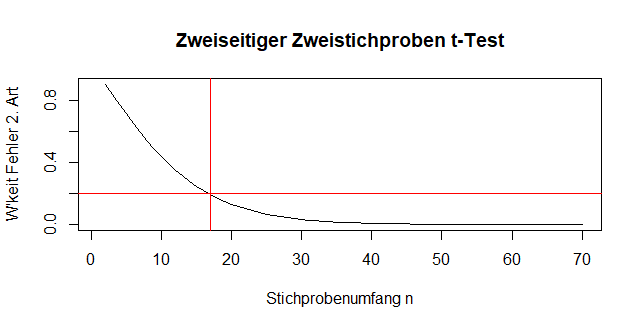
\includegraphics[scale=0.7]{Stichprobenumfang.png}

\end{figure} 

\noindent Bei sechs Messungen mit jeweils 10 Thermometern ergibt sich ein Stichprobenumfang von N=60, für welchen die Wahrscheinlichkeit für einen Beta-Fehler deutlich unter dem Wert von 0.2 liegt und welcher somit gerechtfertigt ist. \\

\noindent Der Erstellung des Plans \ref{Plan} erfolgte mit der Funktion design.crd() aus dem R-Paket \enquote{agricolae}. Für jede der sechs Messungen wurde ein vollständig randomisierter Plan erstellt, wobei, wie oben beschrieben, jeweils 10 Thermometer auf die zwei Faktorstufen \enquote{inside} und \enquote{outside} aufgeteilt wurden. Für jede Durchführung wurde ein anderer Seed gesetzt und die sechs resultierenden Pläne schließlich der Reihenfolge nach auf die zwei Zeitblöcke aufgeteilt. 




\begin{table}[ht]
\caption{Versuchsplan Temperaturexperiment}
\centering
\fbox{
\begin{tabular}{c|c|lll}
  
  4-6 Uhr & Thermometer & 1. Messung & 2. Messung & 3. Messung \\ 
  \hline
&1 & in & in & in \\ 
 & 2 & out & out & out \\ 
  & 3 & out & in & out \\ 
   &4 & out & in & in \\ 
   &5 & in & in & out \\ 
   &6 & in & out & out \\ 
   &7 & in & in & out \\ 
   &8 & in & out & in \\ 
   &9 & out & out & in \\ 
   &10 & out & out & in \\ 
   \hline
   16-18 Uhr & & & & \\
   \hline
  & 1 & out & in & in \\ 
  &2  & out & in & out \\ 
  &3  & in & out & in \\ 
  &4  & in & in & out \\ 
  &5  & out & out & out \\ 
  &6  & in & out & in \\ 
  &7  & in & in & in \\ 
  &8  & in & out & in \\ 
  &9  & out & out & out \\ 
  &10 & out & in & out \\ 
\end{tabular}
}
\end{table}

	
	\newpage
	\section{Versuchsablauf}
	Zunächst muss bestimmt werden, welche Personen Innen/Außen die Thermometer aufstellen und die Messungen ablesen und dokumentieren. \ref{Verteilung}
	\begin{table}[h]
		\begin{tabular}{l|l|l}
			
			Uhrzeit		&	Beschreibung									&	Versuchsleiterin \\
			\hline
			03:30 Uhr	&	Vorbereitung der Messorte						& alle\\
			03:55 Uhr	&	Aufstellen der Thermometer						& D.Grosse-Hering/K.Bayer\\
			04:00 Uhr	&	Beginn der 1.Messung							& \\
			04:20 Uhr	& 	Ende der 1.Messung: dokumentieren, Zwischenlagerung & A.Hemmersbach/K.Gurtskaia\\
			
			04:40 Uhr	&	Aufstellen der Thermometer						&D.Grosse-Hering/K.Bayer\\
			04:45 Uhr	&	Beginn der 2.Messung							& \\
			05:05 Uhr	& 	Ende der 2.Messung: dokumentieren, Zwischenlagerung & A.Hemmersbach/K.Gurtskaia\\
			
			05:25 Uhr	&	Aufstellen der Thermometer						&D.Grosse-Hering/K.Bayer\\
			05:40 Uhr	&	Beginn der 3.Messung							& \\
			06:00 Uhr	& 	Ende der 3.Messung: dokumentieren, Zwischenlagerung & A.Hemmersbach/K.Gurtskaia\\
			
			\hline
			06:20 Uhr	& 	Pause											& alle \\
			\hline
			
			15:55 Uhr	&	Aufstellen der Thermometer						&A.Hemmersbach/D.Grosse-Hering\\
			16:00 Uhr	&	Beginn der 1.Messung							& \\
			16:20 Uhr	& 	Ende der 1.Messung: dokumentieren, Zwischenlagerung &K.Bayer/K.Gurtskaia \\
			
			16:40 Uhr	&	Aufstellen der Thermometer						&A.Hemmersbach/D.Grosse-Hering\\
			16:45 Uhr	&	Beginn der 2.Messung							&K.Bayer/K.Gurtskaia\\
			17:05 Uhr	& 	Ende der 2.Messung: dokumentieren, Zwischenlagerung &\\
			
			17:25 Uhr	&	Aufstellen der Thermometer						&A.Hemmersbach/D.Grosse-Hering\\
			17:40 Uhr	&	Beginn der 3.Messung							& \\
			18:00 Uhr	& 	Ende der 3.Messung: dokumentieren, Zwischenlagerung & K.Bayer/K.Gurtskaia\\
			
			\hline
			
			18:20 Uhr	&	Nachbesprechung									& alle \\
			18:50 Uhr	& 	Digitalisierung der Messdaten					&A.Hemmersbach\\
			
			
		\end{tabular}
	\end{table}
	\newpage
	
	\newpage
	
	\renewcommand{\thesubsection}{\Alph{subsection}}
	
	
	\section{Anhang}
	
	\subsection{Literatur}
	%\bibliography{Literatur}
	\printbibliography[heading=none]

	\subsection{R-Code zum Versuchsplan}\label{Plan}
\lstinputlisting{versuchsplan_temp.R}
\subsection{Bestimmung der Stichprobengröße}\label{Stichprobenumfang}
\lstinputlisting{stichprobengroesse.R}

\newpage
	\subsection{Aufgaben Verteilung} \label{Verteilung}
	
	
	\begin{lstlisting}
		
    Versuchsleiterin <- c("K.Bayer","A.Hemmersbach","D.Grosse-Hering","K.Gurtskaia")
		
    set.seed(1539)

    #Morgens Innen
    sample(Versuchsleiterin,2)
    ## "D.Grosse-Hering" "A.Hemmersbach" 
		
    #Morgens Aussen
    ##"K.Bayer" "K.Gurtskaia"
		
    set.seed(1540)
		
    #Nachmittags Innen
    sample(Versuchsleiterin,2)
    ##"A.Hemmersbach" "K.Bayer"
		
    #Nachmittags Aussen
    ## "D.Grosse-Hering" "K.Gurtskaia"
		
    set.seed(1540)
    #Digitalisierung der Daten
    sample(Versuchsleiterin,1)
    ##"A.Hemmersbach"
	\end{lstlisting}
	
	Die Erstgenannte Person wird für die Aufstellung der Thermometer und die zweitgenannte Person ist für die Dokumentierung der Messdaten zuständig.	
	
	\begin{figure}[t]
		\subsection{Erklärung zum Bericht}
		\hspace{-1.3cm}
		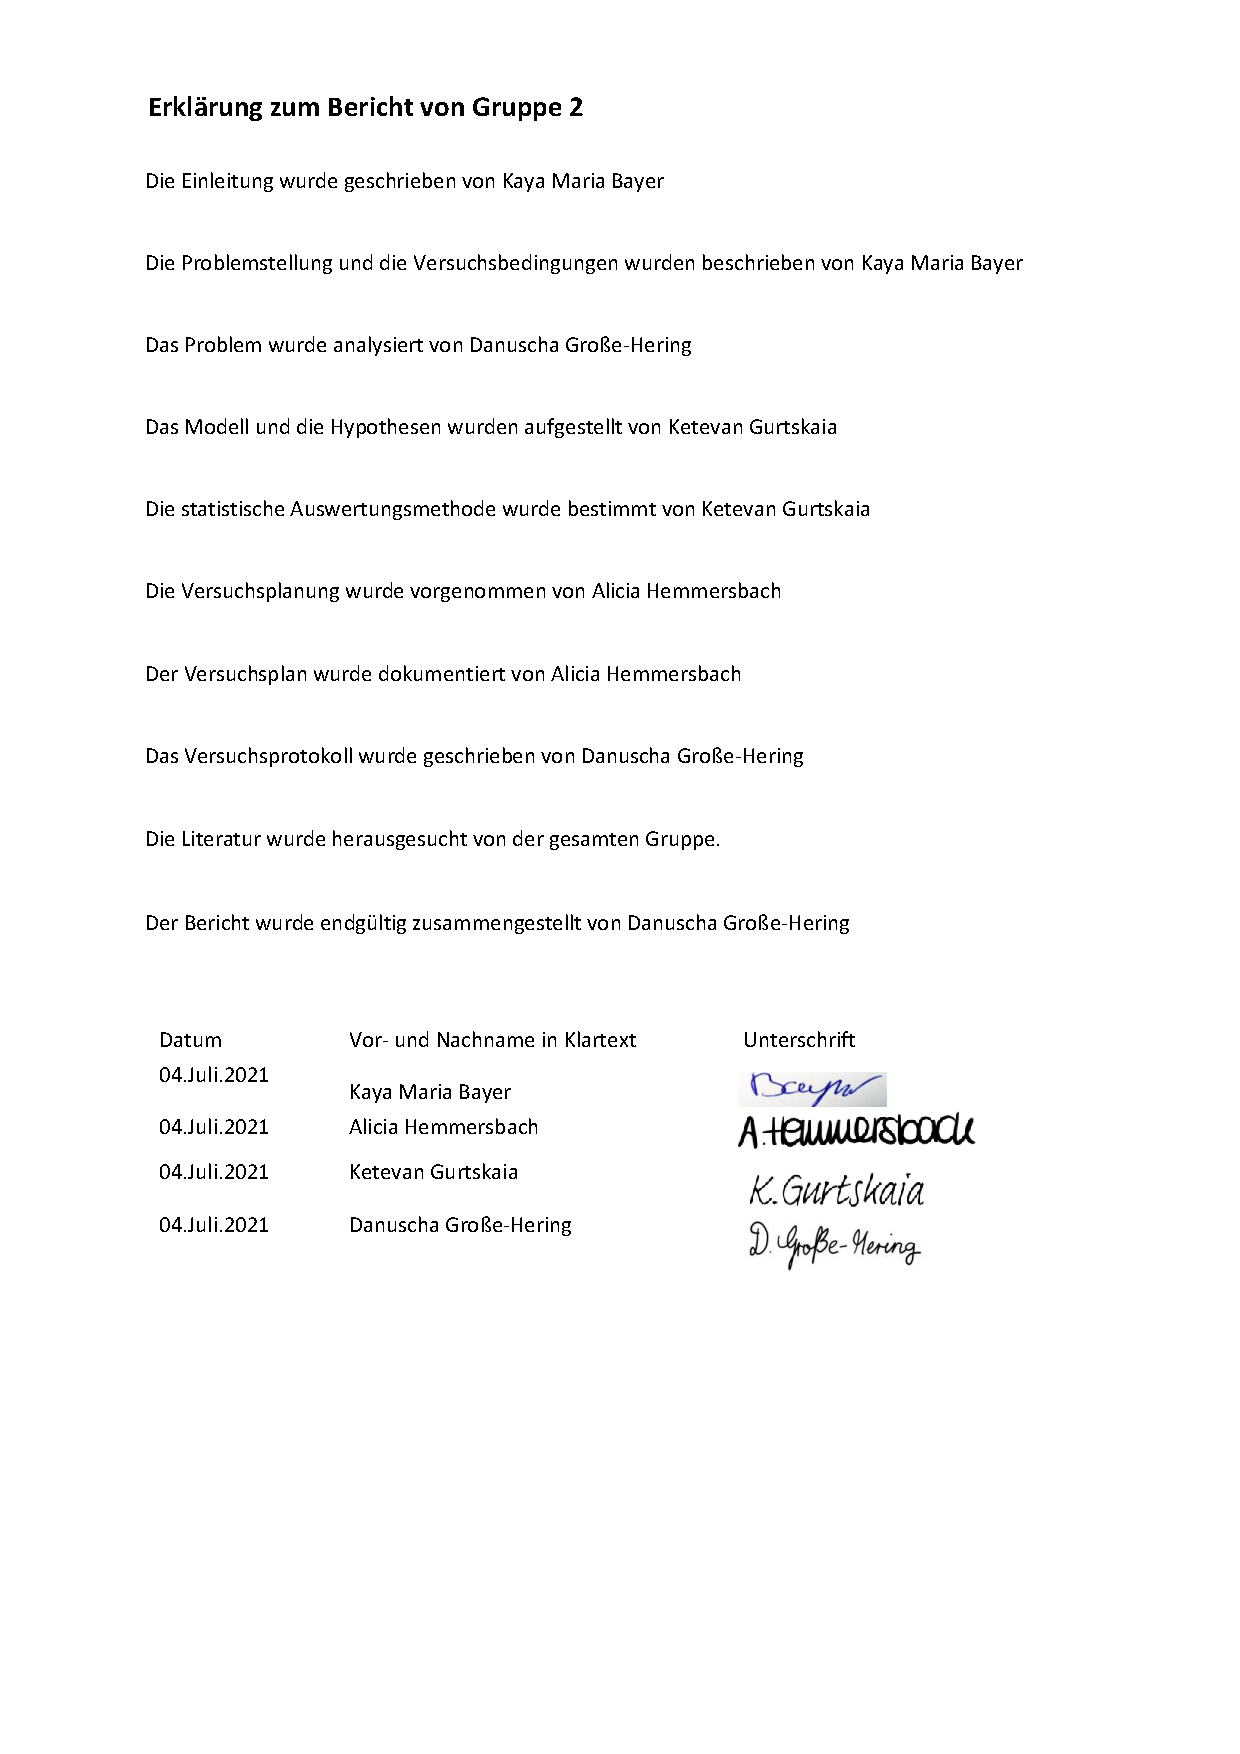
\includegraphics[scale=0.8, page=1]{ErklaerungzumBericht}
	\end{figure}
	
	
\end{document}


